\documentclass{../../../oss-apphys}
%\usepackage{bm}

\begin{document}
\genheader

\gentitle{1}{SIMPLE HARMONIC MOTION}

\genmultidirections

\gengravity

\raggedcolumns
\begin{multicols}{2}
  \begin{enumerate}[leftmargin=18pt]

  \item A 0.40-kg mass hangs on a spring with a spring constant of 12 N/m.
    The system oscillates with a constant amplitude of 12 cm. What is the
    maximum acceleration of the system?
    \begin{enumerate}[noitemsep,topsep=0pt,leftmargin=18pt,label=(\Alph*)]
    \item\SI{0.62}{m/s^2}
    \item\SI{1.4}{m/s^2}
    \item\SI{1.6}{m/s^2}
    \item\SI{3.6}{m/s^2}
    \item\SI{9.8}{m/s^2}
    \end{enumerate}

  \item A mass is attached to a spring and allowed to oscillate vertically.
    Which of the following would NOT change the period of the oscillation?
    \begin{enumerate}[noitemsep,topsep=0pt,leftmargin=18pt,label=(\Alph*)]
    \item Double the mass and double the spring constant
    \item Double the amplitude of vibration and double the mass
    \item Double the gravitational field strength and double the mass
    \item Double the gravitational field strength and double the spring constant
    \item Double the gravitational field strength and quadruple the mass
    \end{enumerate}
      
  \item The Moon is approximately \SI{384000}{\kilo\metre} from the Earth. The
    Moon revolves around the Earth once every 27.3 days. What is the frequency
    of the Moon's motion?
    \begin{enumerate}[noitemsep,topsep=0pt,leftmargin=18pt,label=(\Alph*)]
    \item \SI{14100}{km} each day
    \item 0.0366 revolution each day
    \item 0.036630 revolution each day
    \item 655 hours for each revolution
    \item 27.3 days for each revolution
    \end{enumerate}

  \item A mass is suspended from a spring and allowed to oscillate freely. When
    the amplitude of vibration is doubled, what happens to frequency of
    vibration?
    \begin{enumerate}[noitemsep,topsep=0pt,leftmargin=18pt,label=(\Alph*)]
    \item It quadruples.
    \item It doubles.
    \item It stays the same.
    \item It reduces to one-half of what it was.
    \item It reduces to one-fourth of what it was.
    \end{enumerate}
    

    
    \columnbreak
    
  \item A bell is rung when the dangling clapper within it makes contact with
    the bell. A poorly designed bell has a clapper that swings with the same
    period as the bell. How can this design be improved?
    \begin{enumerate}[noitemsep,topsep=0pt,leftmargin=18pt,label=(\Alph*)]
    \item Use a clapper with a smaller mass on the end so it is out of period
      with the bell.
    \item Use a clapper with a bigger mass on the end so it is out of period
      with the bell.
    \item Force the bell to swing with greater amplitude.
    \item Use a longer clapper so it is out of period with the bell.
    \item Increase the mass of the bell so it makes better contact with the
      clapper.
    \end{enumerate}
%155. A meter stick is held at one end by a frictionless pivot and is held
%horizontally at the other end. Neglecting air resistance, how far will the
%meter stick swing when released?
%
%(A) It will swing in a circle around the pivot and back to the starting
%point.
%(B) It will swing just short of horizontal on the other side of the pivot.
%(C) It will swing just beyond horizontal on the other side of the pivot.
%(D) It will swing to horizontal on the other side of the pivot.
    %(E) It will drop to vertical and stop.

  \item  A toy nicknamed the ``Newton’s cradle'' consists of five steel balls,
    each suspended by two strings and each touching the adjacent ball(s).
    When a ball at the end is raised and then dropped, it hits the adjacent
    ball and the ball at the other end rises. Why?
    \begin{enumerate}[noitemsep,topsep=0pt,leftmargin=18pt,label=(\Alph*)]
    \item The elastic energy of the moving ball is transferred to chemical
      energy.
    \item The potential energy of the center balls keeps them in place.
    \item The kinetic energy of the moving ball is transferred through theset
      of balls causing the ball at the end to rise up.
    \item The potential energy of the moving ball is transferred through the
      set of balls to the only ball that can move, causing it to rise.
    \item The center balls are glued together and do not move.
    \end{enumerate}
    \columnbreak
    
  \item Which choice below best explains why a pendulum does not oscillate
    in zero gravity?
    \begin{enumerate}[noitemsep,topsep=0pt,leftmargin=18pt,label=(\Alph*)]
    \item The pendulum has no mass in zero gravity.
    \item A pendulum requires gravity to create the restoring force.
    \item The pendulum is in orbit and considered weightless.
    \item The pendulum would be too far from the Earth to work properly.
    \item The pendulum must have an oscillating tension in the string to
      function properly.
    \end{enumerate}
    
%158. Some large oil tankers have an antiroll water tank inside the hull that
%matches the resonant frequency of the ship’s hull. When ocean waves
%hit the ship at the resonant frequency, how does the water tank prevent
%the ship from capsizing in the waves?
%(A)
%(B)
%(C)
%(D)
%(E)
%The energy of the waves is used by the water in the tank.
%The waves enter the tank and are dampened.
%The water tank is 180° out of phase with the ship’s hull.
%The water tank is 90° out of phase with the ship’s hull.
%The water in the tank is in phase with the ship’s hull.

%159. A pendulum has a bob of 28 kg and is 38 cm in diameter. It is hung on
%a wire that is 67 m long. What are its period and frequency near the
%surface of the Earth?
%(A)
%(B)
%(C)
%(D)
%(E)
%0.061 s and 16 cycles/s
%16 s and 0.061 cycle/s
%0.60869 s and 16.429 cycles/s
%11 s and 0.094 cycle/s
%0.094 s and 11 cycles/s

%160. One end of a 50-kg mass is attached to two vertical springs in parallel.
%Each spring has a spring constant of 20 N/m. When the spring is pulledback and released, what is the system’s period?
%(A)
%(B)
%(C)
%(D)
%(E)
%14.04962946 s
%7.024814731 s
%14 s
%7.0 s
%0.14 s
%    
%161. A mass of 50 kg is held vertically by two springs, one connected to the
%other in series. Each spring has a spring constant of 20 N/m. When set
%in motion, what is the system’s period?
%(A)
%(B)
%(C)
%(D)
%(E)
%0.14 s
%14 s
%7.0 s
%14.04962946 s
%7.024814731 s
%162. A mass of 50 kg is held horizontally on a frictionless surface by two
%springs, one at each end of the mass. Each spring has a spring constant
%of 20 N/m. When set in motion, what is the system’s period?
%(A)
%(B)
%(C)
%(D)
%(E)
%14.04962946 s
%7.024814731 s
%14 s
%7.0 s
%0.14 s
%163. A mass of 50 kg is held horizontally on a frictionless surface by two
%springs, one connected to the other in series. Each spring has a spring
%constant of 20 N/m. When set in motion, what is the system’s period?
%(A)
%(B)
%(C)
%(D)
%(E)
%0.14 s
%14 s
%7.0 s
%14.04962946 s
%7.024814731 s
%164. A 10-kg mass is placed on a frictionless surface and attached to aspring that is attached to a fixed wall. The spring’s constant is 20 N/m.
%When set in motion, what is the system’s period, and what is the period
%if the system is held vertically?
%(A)
%(B)
%(C)
%(D)
%(E)
%4.4 s and 8.9 s
%8.885765876 s for both
%8.885765876 s and 17.77153175 s
%4.4 s for both
%13 s for both
%165. A 15-kg mass rests on two springs and is held by a spring attached to
%the ceiling. The spring constant for each of the bottom two springs is 10
%N/m, and the spring constant for the upper spring is 25 N/m. When set
%in motion, what is the system’s period?
%(A)
%(B)
%(C)
%(D)
%(E)
%3.6 s
%7.2 s
%1.8 s
%1.2 s
%The mass will not move.
%166. A mass of 12 kg is hung onto a spring attached to the ceiling. The
%spring’s constant is 19 N/m. How far will the spring stretch when the
%weight is hung, and what will be the system’s period when activated?
%(A)
%(B)
%(C)
%(D)
%(E)
%6.2 cm and 15 s
%6.2 m and 5 min
%62 mm and 15.6 s
%6.2 m and 5.0 s
%6.2 m and 156 s


  \item A refrigerator compressor that weighs 8 kg is fixed to three separate
    springs on the refrigerator frame. Each has a spring constant of 0.01
    N/m. What is the natural frequency of the system?
    \begin{enumerate}[noitemsep,topsep=0pt,leftmargin=18pt,label=(\Alph*)]
    \item 0.01 cycle/s
    \item 0.03 cycle/s
    \item 0.8 cycle/s
    \item 103 cycles/s
    \item 0.003 cycle/s
    \end{enumerate}
    
%168. The pendulum on an old mechanical, weight-driven clock has a period
%of 3.0 s. What is the length of the clock’s pendulum?
%(A)
%(B)
%(C)
%(D)
%(E)
%2.2 m
%3.5 m
%22 cm
%35 cm
%3.0 m
%169. A blue light wave vibrates at 6.98 × 10 14 Hz. What is its period of
%vibration?
%(A)
%(B)
%(C)
%(D)
%(E)
%6.98 × 10 14 s
%1.43 × 10 -15 s
%2.09 × 10 23 m/s
%3.00 × 10 8 m/s
%2.09 × 10 23 m
%170. A steel ball with a mass of 100 g is dropped onto a steel plate. The
%collision is perfectly elastic. From what height must the ball be dropped
%for the vibrating system to have a bounce period of 2.0 s?
%(A)
%(B)
%(C)
%(D)
%(E)
%100. cm
%20. m
%0.10 m
%9.8 m
    %4.9 m
    
  \item A pendulum on the surface of the Moon has a period of 1.0 s. If the
    length of the pendulum is quadrupled, what is the value of the new
    period?
    \begin{enumerate}[noitemsep,topsep=0pt,leftmargin=18pt,label=(\Alph*)]
    \item 0.25 s
    \item 0.50 s
    \item 1.0 s
    \item 2.0 s
    \item 4.0 s
    \end{enumerate}
    
  \item A 2.0-m pendulum on a particular planet has a period of 4.6 s. What is
    the gravitational field strength on that planet?
    \begin{enumerate}[noitemsep,topsep=0pt,leftmargin=18pt,label=(\Alph*)]
    \item 1.6 N/kg
    \item 3.7 N/kg
    \item 4.9 N/kg
    \item 9.8 N/kg
    \item 25 N/kg
    \end{enumerate}
%173. A particle oscillates with simple harmonic motion with no damping.
%Which one of the following statements about the acceleration of the
%oscillating particle is true?
%(A)
%(B)
%(C)
%(D)
%(E)
%It has a value of 9.8 m/s 2 when the oscillation is vertical.
%It is zero when the speed is the minimum.
%It is proportional to the frequency.
%It is zero throughout the oscillation.
    %It is zero when the speed is the maximum.
    \columnbreak
    
  \item The displacement (in centimeters) of the vibrating cone of a large
    loudspeaker is represented by the equation $\Delta x=2.0\cos(150t)$, where
    $t$ is the time in seconds. What distance does the tip of the cone move in
    half a period?
    \begin{enumerate}[noitemsep,topsep=0pt,leftmargin=18pt,label=(\Alph*)]
    \item 0.007 cm
    \item 1.0 cm
    \item 2.0 cm
    \item 4.0 cm
    \item 150 cm
    \end{enumerate}
%175. The displacement (in centimeters) of the vibrating cone of a large
%loudspeaker is represented by the equation $\Delta x = 2.0 \cos(150t)$. What is
%the frequency of the vibration of the tip of the cone?
%(A) 24 Hz
%(B) 0.042 Hz
%(C) 150 Hz(D) 2.0 Hz
%(E) 1.0 Hz

  \item The graph below shows the displacement versus time for an object. Which
    equation best describes its displacement in meters?\\
    \pic{.45}{d-t}
    \begin{enumerate}[noitemsep,topsep=0pt,leftmargin=18pt,label=(\Alph*)]
    \item $\Delta x=20\cos(0.5t)$
    \item $\Delta x=10\cos(2t)$
    \item $\Delta x=10\cos(\pi t)$
    \item $\Delta x=20\cos(2t)$
    \item $\Delta x=20\sin(\pi t)$
    \end{enumerate}

  \item The Moon has a gravitational field strength that is approximately
    one-sixth of the field on the Earth. What is the ratio between the period
    of a pendulum on the Moon and the period of an identical pendulum on the
    Earth?
    \begin{enumerate}[noitemsep,topsep=0pt,leftmargin=18pt,label=(\Alph*)]
    \item 6
    \item $\sqrt{6}$
    \item $\displaystyle\frac16$
    \item $\displaystyle\frac1{\sqrt{6}}$
    \item 1
    \end{enumerate}
  \end{enumerate}
  \columnbreak

  \textbf{Questions \ref{one}--\ref{four}} are based on the figure below of a
  mass-spring system. Assume the mass is pulled back to position +A and
  released, and it slides back and forth without friction.
  \begin{center}
    \pic{.3}{springs}
  \end{center}
  \begin{enumerate}[leftmargin=18pt,resume]
  \item When the mass reaches position $-A$, what can be said about its speed?
    \label{one}
    \begin{enumerate}[noitemsep,topsep=0pt,leftmargin=18pt,label=(\Alph*)]
    \item It is a minimum.
    \item It is a maximum.
    \item It is zero.
    \item It is decreasing.
    \item It is increasing.
    \end{enumerate}
    
  \item When the mass reaches position 0, what can be said about its speed?
    \begin{enumerate}[noitemsep,topsep=0pt,leftmargin=18pt,label=(\Alph*)]
    \item It is a minimum.
    \item It is a maximum.
    \item It is zero.
    \item It is decreasing.
    \item It is increasing.
    \end{enumerate}
    
  \item At what position does the mass have the greatest acceleration?
    \begin{enumerate}[noitemsep,topsep=0pt,leftmargin=18pt,label=(\Alph*)]
    \item $-A$
    \item $-A/2$
    \item 0
    \item $+A/2$
    \item $+A$
    \end{enumerate}
    
  \item The mass is released from the $-A$ position at time $t=0$, and it
    oscillates with period $T$, measured in seconds. Which equation best
    represents the displacement?
    \label{four}
    \begin{enumerate}[noitemsep,topsep=0pt,leftmargin=18pt,label=(\Alph*)]
    \item $\displaystyle \Delta x = -A\cos\left(\frac{T}{2\pi}t\right)$
    \item $\displaystyle \Delta x = -(A/2)\cos(2\pi T t)$
    \item $\displaystyle \Delta x = -A\cos\left(\frac{2\pi}{T}t\right)$
    \item $\displaystyle \Delta x = (A/2)\cos(T t)$
    \item $\displaystyle \Delta x = A\cos\left(\frac{2\pi}{T}t\right)$
    \end{enumerate}
    
%181. A mass-spring system oscillates up and down in a gravitational field.When is its kinetic energy the greatest?
%(A)
%(B)
%(C)
%(D)
%(E)
%When it’s passing through equilibrium
%At the top of its motion
%At the bottom its motion
%When its gravitational potential energy is the greatest
%When its elastic energy is the greatest
   
  \end{enumerate}
  \columnbreak
  
  For questions \ref{multi-1st}--\ref{multi-last}, two of the suggested answers
  will be correct. Select the two best answers, and record them both on the
  answer sheet.
  \begin{enumerate}[leftmargin=18pt,resume]
  \item Which of the following are NOT examples of simple harmonic motion?
    \label{multi-1st}
    \begin{enumerate}[noitemsep,topsep=0pt,leftmargin=18pt,label=(\Alph*)]
    \item A tennis ball bouncing on the ground
    \item A child swinging freely back and forth in a toddler swing
    \item A plucked guitar string
    \item A child who continues to jump up and down
    \item A ball rolling back and forth in a bowl
    \end{enumerate}

  \item Which of the following best represent periodic motion?
    \begin{enumerate}[noitemsep,topsep=0pt,leftmargin=18pt,label=(\Alph*)]
    \item A skydiver who has reached terminal velocity
    \item The Moon in orbit about the Earth
    \item A car driving to each state in the United States
    \item A cart pushed up a frictionless incline plane
    \item A pendulum swinging over a 30-min time span.
    \end{enumerate}
    
  \item  Which of the following significantly affect the period of a simple
    pendulum?
    \begin{enumerate}[noitemsep,topsep=0pt,leftmargin=18pt,label=(\Alph*)]
    \item The length of the pendulum
    \item The mass of the pendulum bob
    \item The amplitude of swing
    \item The gravitational field strength
    \item The thickness of the string
    \end{enumerate}
    
  \item A mass is suspended from a vertical spring attached to a support. Which
    of the following significantly affect the frequency of oscillation of this
    system?
    \begin{enumerate}[noitemsep,topsep=0pt,leftmargin=18pt,label=(\Alph*)]
    \item The spring constant
    \item The gravitational field strength
    \item The value of the mass
    \item Friction between the mass and the spring
    \item The surface area of the mass
    \end{enumerate}
    
  \item A mass oscillates from the end of a vertical spring. What may be done
    to increase the frequency of oscillation?
    \label{multi-last}
    \begin{enumerate}[noitemsep,topsep=0pt,leftmargin=18pt,label=(\Alph*)]
    \item Increase the mass
    \item Decrease the mass
    \item Increase the spring constant
    \item Increase the strength of the gravitational field
    \item Increase the amplitude of vibration
    \end{enumerate}
  \end{enumerate}
\end{multicols}

%\newpage
%\begin{center}
%  {\Large
%    \textbf{AP\textsuperscript{\textregistered} Physics 1 \&C: Circular Motion\\
%      Student Answer Sheet for Multiple-Choice Section}
%  }
%  
%%  \begin{minipage}[t]{.3\textwidth}
%  \vspace{.2in}
%  \bgroup
%  \begin{tabular}{>{\centering}m{1.3cm} >{\centering}m{1.7cm}}
%    No. & Answer
%  \end{tabular}\\
%  \def\arraystretch{1.5}
%  \begin{tabular}{|>{\centering}m{1.3cm}|>{\centering}m{1.7cm}|}
%    \hline
%    1 & \\ \hline
%    2 & \\ \hline
%    3 & \\ \hline
%    4 & \\ \hline
%    5 & \\ \hline
%    6 & \\ \hline
%    7 & \\ \hline
%    8 & \\ \hline
%    9 & \\ \hline
%    10 & \\ \hline
%    11 & \\ \hline
%    12 & \\ \hline
%    13 & \\ \hline
%    14 & \\ \hline
%    15 & \\ \hline
%    16 & \\ \hline
%    17 & \\ \hline
%    18 & \\ \hline
%    19 & \\ \hline
%    20 & \\ \hline
%    21 & \\ \hline
%    22 & \\ \hline
%%    23 & \\ \hline
%%    24 & \\ \hline
%%    25 & \\ \hline
%  \end{tabular}
%  \egroup
%%  \end{minipage}
%%  \begin{minipage}[t]{.3\textwidth}
%%  \vspace{.2in}
%%  \bgroup
%%  \begin{tabular}{>{\centering}m{1.3cm} >{\centering}m{1.7cm}}
%%    No. & Answer
%%  \end{tabular}\\
%%  \def\arraystretch{1.5}
%%  \begin{tabular}{|>{\centering}m{1.3cm}|>{\centering}m{1.7cm}|}
%%    \hline
%%    26 & \\ \hline
%%    27 & \\ \hline
%%    28 & \\ \hline
%%    29 & \\ \hline
%%    30 & \\ \hline
%%    31 & \\ \hline
%%    32 & \\ \hline
%%    33 & \\ \hline
%%    34 & \\ \hline
%%    35 & \\ \hline
%%    36 & \\ \hline
%%    37 & \\ \hline
%%    38 & \\ \hline
%%  \end{tabular}
%%  \egroup
%%  \end{minipage}
%\end{center}
\newpage

\genfreetitle{1}{CIRCULAR MOTION AND SIMPLE HARMONIC MOTION}{3}

\genfreedirections

% QUESTION IS TAKEN FROM 2018 AP PHYSICS 1 FREE-RESPONSE QUESTION #5
\begin{center}
  \pic{.5}{blocks}
\end{center}
\begin{enumerate}[leftmargin=15pt]
\item (7 points, suggested time 13 minutes) Block $P$ of mass $m$ is on a
  horizontal, frictionless surface and is attached to a spring with spring
  constant $k$. The block is oscillating with period $T_P$ and amplitude $A_P$
  about the spring's equilibrium position $x_0$. A second block $Q$ of mass
  $2m$ is then dropped from rest and lands on block $P$ at the instant it
  passes through the equilibrium position, as shown above. Block $Q$
  immediately sticks to the top of block $P$, and the two-block system
  oscillates with period $T_{PQ}$ and amplitude $A_{PQ}$.
  \begin{enumerate}[leftmargin=18pt]
  \item Determine the numerical value of the ratio $T_{PQ}/T_P$.
    \vspace{1in}
  \item How does the amplitude of oscillation $A_{PQ}$ of the two-block system
    compare with the original amplitude $A_P$ of block $P$ alone?

    \vspace{.1in}
    \underline{\hspace{.3in}} $A_{PQ}<A_{P}$\hspace{.25in}
    \underline{\hspace{.3in}} $A_{PQ}=A_{P}$\hspace{.25in}
    \underline{\hspace{.3in}} $A_{PQ}>A_{P}$

    \vspace{.2in}In a clear, coherent paragraph-length response that may also
    contain diagrams and/or equations, explain your reasoning.
  \end{enumerate}
  \newpage
  
\item In heavy seas, the bow of a battle ship undergoes a simple harmonic
  vertical pitching motion with a period of \SI{8.}{\second} and an amplitude
  of \SI{2.}{\metre}.
  \begin{enumerate}[leftmargin=18pt]
  \item What is the maximum vertical velocity of the battle ship's bow?
  \item What is its maximum acceleration?
  \item An \SI{80}{\kilo\gram} sailor is standing on the scale in the bunk room
    in the bow. What are the maximum and minimum reading on the scale in
    newtons?
    \vspace{.8in}
  \end{enumerate}

\item Show that for the situations in the figures below, the object of mass
  $m$ oscillates with a frequency of
  $\displaystyle f=\frac{1}{2\pi}\sqrt{\frac{k_\mathrm{eff}}{m}}$
  where $k_\mathrm{eff}$ is given by (a) $k_\mathrm{eff}=k_1+k_2$ and (b)
  $\displaystyle\frac{1}{k_\mathrm{eff}}=\frac{1}{k_1}+\frac{1}{k_2}$. Hint:
  find the net force on the mass and write $F=-k_\mathrm{eff}x$. Note that in
  (b), the springs stretch by different amounts, the sum of which is $x$.
  
  (a)\hspace{5pt}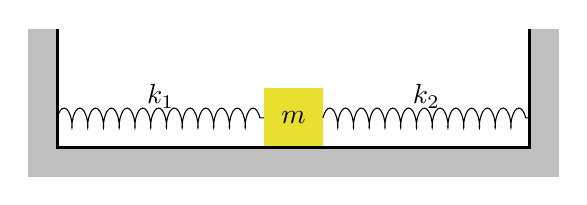
\begin{tikzpicture}[scale=.5]
    \fill[gray!50](0,0) rectangle(12,-.75);
    \fill[gray!50](-.75,-.75) rectangle(0,3);
    \fill[gray!50](12,-.75) rectangle(12.75,3);
    \fill[yellow!80!gray](5.25,0) rectangle(6.75,1.5) node[midway,black]{$m$};
    \draw[decoration={aspect=0.3,segment length=2mm, amplitude=1.25mm, coil},
      decorate] (0,.75)--(5.25,.75) node[midway,above]{$k_1$};
    \draw[decoration={aspect=0.3,segment length=2mm, amplitude=1.25mm, coil},
      decorate] (6.75,.75)--(12,.75) node[midway,above]{$k_2$};
    \draw[very thick](0,3)--(0,0)--(12,0)--(12,3);
  \end{tikzpicture}

  (b)\hspace{5pt}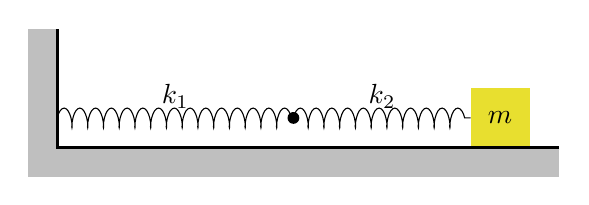
\begin{tikzpicture}[scale=.5]
    \fill[gray!50](0,0) rectangle(12.75,-.75);
    \fill[gray!50](-.75,-.75) rectangle(0,3);
    \fill[yellow!80!gray](10.5,0) rectangle(12,1.5) node[midway,black]{$m$};
    \draw[decoration={aspect=0.3,segment length=2mm, amplitude=1.25mm, coil},
      decorate] (0,.75)--(6,.75) node[midway,above]{$k_1$};
    \draw[decoration={aspect=0.3,segment length=2mm, amplitude=1.25mm, coil},
      decorate] (6,.75)--(10.5,.75) node[midway,above]{$k_2$};
    \fill[black](6,.75) circle(.15);
    \draw[very thick](0,3)--(0,0)--(12.75,0);
  \end{tikzpicture}
  \vspace{3in}
  \newpage
  
\item A simple pendulum of length $L$ is released from rest from an angle of
  $\theta_0$.
  \begin{enumerate}[itemsep=.8in,topsep=0pt,leftmargin=15pt]
  \item Assuming the motion of the pendulum to be simple harmonic motion, find
    its speed as it passes through $\theta=0$.
  \item Using the conservation of energy, find this speed exactly.
  \item Show that your results for (a) and (b) are the same when $\theta_0$ is
    small.
  \item Find the difference in your results for $\theta_0=\SI{.20}{rad}$ and
    $L=\SI{1}{\metre}$.
  \end{enumerate}
 
\end{enumerate}
\end{document}
